\documentclass{article}
\usepackage[utf8]{inputenc}
\usepackage[]{tikz}
\usepackage{mathtools}
\usepackage{circuitikz} 
\usepackage{float}
\usepackage[]{graphicx}
\title{Discrete Time Control System}
\author{Deependra Neupane}

\begin{document}

\section{Introduction:}
We are already been familiar with continuous time system which uses the continuous time signals. Continuous time signal is defined in every range of time. It can take continuous or definite values of amplitude over a continuous range of time. We write continuous time signals as function of time, x(t). Analog signal are quite different than continuous time signal, since it is an special case of continuous time signals whose amplitude can take a continuous range of values.

In contrast to continuous time system, discrete time system uses discrete time signals which have the amplitudes for only a distinct points in time but it can assume continuous range of values of amplitudes. If the amplitude takes continuous values then the signal is called sampled data signal but the signal that takes only quantized values of amplitude then it is called digital signal.In discrete time signal, time is a discrete variable. We write the discrete time signals as a function of integer n, x(n). The process of representing a variable by a set of distinct values is called quantization and the resulting distinct values are called quantized values. They changes only by a set of distinct values. The term quantized values should not be confused with sampled data, since, sampled data signal takes a continuous range of values and it is generated by sampling an analog signal at discrete instants of time. In general sampled data signal is an amplitude modulated pulse signals. So, a digital signal is a discrete time signal that have the quantized amplitude.

Discrete time control systems are the control system in which one or more variables can change only at discrete instants of time. The time at which the value changes is denoted by kT, where k = 0,1,2,3...... This represents time at which some physical measurement is done or at which the memory of a digital computer is read out.
The sampled data from the analog signal needs to be converted in to digital signal if there involves any digital computer the processes the signal.
\begin{figure}[H]
	\begin{tikzpicture}
	\draw[thick, ->] (0,0) --(4,0) node[anchor = north west]{t};
	\draw[thick,->] (0,0) -- (0,4) node[anchor = south east]{x(t)};
	\draw plot [smooth, tension=1] coordinates { (0,1) (1,1) (2,3) (3,1)};
	
	\end{tikzpicture}
	
	\caption{Continuous time signal}
\end{figure}[H]
\begin{figure}
		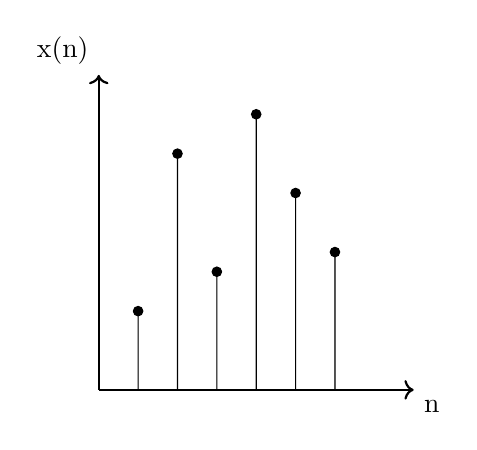
\begin{tikzpicture}
	\draw[thick, ->] (0,0) --(4,0) node[anchor = north west]{n};
	\draw[thick,->] (0,0) -- (0,4) node[anchor = south east]{x(n)};
	
	\draw[fill ](0.5,0) -- (0.5,1) circle[radius=0.06]; 
	\draw[fill ](1,0) -- (1,3) circle[radius=0.06]; 
	\draw[fill ](1.5,0) -- (1.5,1.5) circle[radius=0.06]; 
	\draw[fill ](2,0) -- (2,3.5) circle[radius=0.06]; 
	\draw[fill ](2.5,0) -- (2.5,2.5) circle[radius=0.06]; 
	\draw[fill ](3,0) -- (3,1.75) circle[radius=0.06]; 
	
	\end{tikzpicture}
	\caption{Discrete time signal}
\end{figure}

	

\newpage
\paragraph{Sampling:}
The sampling of the continuous time signals or analog signal converts the original signal to a sequence of values at discrete time points.If there involves any digital controller, it is required to do sampling and quantize amplitude values, in other words, to make digital signal that corresponds to input continuous time signal. For example, if we want to measure the voltage of generated by a solar panel, then voltage signals can be sampled for every 1 minute. This sampled values are now quantized by quantization process which process the sampled analog signal and gives digital amplitude signal, i.e set of binary numbers. These set of binary numbers are now processed by the digital controller and gives a digital output which is sent out to hold circuit. The output of the hold circuit is continuous time signal. Sampling operation can be different types. They ar:
\begin{enumerate}
	\item Periodic sampling: the sampling instants are equally spaced ie $t_k = kT$.
	\item Multiple order sampling: The pattern of the $t_k$ is repeated ie $t_{k-r} - t_k$ is constant.
	\item Multiple rate sampling: 
	\item Random sampling:
\end{enumerate}
\paragraph{Reconstruction of Signal}
The reconstruction of the signal produced by the digital controller can be done by using hold circuits. The space between the samples need to be filled before they are sent to the plant or any transducer. The hold circuits are designed to extrapolate the output signal between successive points according to some prescribed manner.  There are different types of hold circuit on the basis of their nature of extrapolation. One of the simple type is zero order hold. It basically generates the staircase output by holding a value up to the time interval.
\section{Components of Digital Control System:}
Discrete time control system is basically the combination of continuous and digital system, since the input and output both are in continuous form. The error signal between input and output signal is converted in to digital form by \textbf{sample and hold circuit} and analog to digital converter. The conversion is done in sampling time. Then the digital computer some algorithm to convert the input signal to another output signal. This output signal is now converted in to output continuous signal by using digital to analog converter and hold circuit. The output of the hold circuit is directly fed to plant or transducer.
Note: The process that transforms continuous time signal into discrete time data is called \textbf{sampling or discretization} and the reverse operation that converts the discrete time signal to continuous time signal is called \textbf{data hold}. There are various types of data hold circuit on the basis of their order and done usually by extrapolation methods.

\textbf{Analog to digital converter} is also called encoders. It is a device that converts analog signal into a digital signal. Similarly, digital to analog converters, also called decoders, is a device that converts the digital signal to analog signals.

\textbf{Plant} is any physical object that is to be controlled. And \textbf{transducer} is a device that converts one form of energy to another form. Plant my involve servo system, furnace, a spacecraft. Similarly, transducer may be a thermocouple that converts the temperature difference in to voltage.


\section{Discrete time control system:}
The control design process
\begin{enumerate}
	\item Obtaining the model of the plant ot be controlled typically a transfer function expressed in s.
	\item Choose the performance criteria that the controller must meet: settling time, overshoot etc.
	\item Design a compensator using the method of your choice: root locus, Bode plot etc
	\item Implement the compensator
	\item Evaluate the performance of a compensator against design criteria. If there is not a good match then revisit steps 2-5.
\end{enumerate}


There are different types of compensator, they are lead, lag, lead-lag and so on.
The compensator or so called any function they are nothing but a computer. Since they process the input and generate the output. So what? You will build the ladders of capacitors and inductors and resistors, certainly not you will program in a computer.
Why digital?
It is lot cheaper, you can re flash, you can interface display pushbuttons, communications and so on. Many sensors have digital outputs. Micro controller have many functions.
You have the transfer function. So what is S?
\begin{figure}[h]
	\begin{circuitikz} \draw
		(0,0) -- (2,0)--(2,1)--(3,1) to[resistor, l= $R_1$](4,1)--(5,1)--(5,-1)
		(2,0)--(2,-1)--(3,-1) to[capacitor, l_=C](4,-1)--(5,-1)
		(5,0)-- (8,0)
		(6,0)--(6,-1)to[resistor, l = $R_2$](6,-2)--(6,-3) --(0,-3)--(8,-3)
		(0,-1.5) node{$v_i(t)$}
		(8,-1.5) node{$v_o(t)$}
		;
	\end{circuitikz}
\end{figure}
\break
The circuit equations for this circuit can be determined as:
\break
The equivalent impedance of $R_1$ and C is:
\[  Z_c = R_1 // \frac{1}{sC}
\]

\[ Z_c = \frac{R_1}{1 + sCR_1}\]
\[ v_i(t) = i(Z_c + R_2)  \]
\[ i(t) = \frac{v_o(t)}{R_2} \]
\[ v_i(t) = (Z_c + R_2) \frac{v_o(t)}{R_2} \]
\[ \frac{v_o(t)}{v_i(t)} = \frac{Z_c + R_2}{R_2} = \frac{R_1 + R_2 + scR_1 R_2}{R_2(1 + sCR_1)} \]
So, we can write 
\[ v_o(t) (s + a) = v_i(t) (s+b)\]
i.e,\[ s v_o(t) + a v_o(t) = s v_i(t) + b v_i(t)\]

We are already familiar with laplace transform. One of the property of Laplace Transform suggests that the multiplication of s with a function in s domain is equivalent to the derivative in time domain.i.e \[sX = \frac{dx}{dt}\]So, what is the derivative of function in discrete system. It is given by:
\[ slope = \frac{v_k - v_{k-1}}{\Delta _T}\]
Note:
\[\frac{dx}{dt} =  \frac{x_k - x_{k-1}}{\Delta_T}\]

\[\frac{d^2 x}{dt^2} =  \frac{x_k - 2 x_{k-1} + x_{k-2}}{\Delta_T ^2}\]
If
\[ u(s) = \frac{y(s)}{s} \Rightarrow  \int y(t) = u(t) \Rightarrow u_k = u_{k-1} + \Delta_T y_k \]
This is called backward Euler integration
\[u_k = u_{k-1} + \Delta_T y_{k-1} + \frac{\Delta_T}{2} (y_k - y_{k-1}) \]
And this is called trapezoidal integration. This is more accurate than that of backward Euler integration. It is used in Tustin Transform.\newline
	Hence, we can replace the s by the above term in discrete time system, so:
\[ \frac{v_{ok} - v_{o(k-1)}}{\Delta _T} + av_o(t)= \frac{v_{ik} - v_{i(k-1)}}{\Delta _T} + bv_i(t) \]

The output voltage is can be written as the function of $v_{ik}$, $v_{i(k-1)}$ and $v_{o(k-1)}$. What this representing is that, the output function at any instant is depending upon previous output, present and previous input. This type of equation is called difference equation. And this is recursive. This provides a great advantage of the modern computers. If we need certain compensator, we are not going to make the complex circuit diagram rather, develop a program algorithm that manipulates the input as same that of the original circuit and use it in a micro controller like raspberry pi.

Difference equations are very important. One of the great example of difference equation is Fibbonaci series. It can be written as:
\[ F_k = F_{k-1} + F_{k-2}\]
One of the revolution in discrete control system is Babbage difference engine which was made in 1823.

Let us introduce the term shift operator ($z^{-1}$) and what the operator does is, it delays the signal by some time value.
\[x_{k-1} = z^{-1}x_k\]
This notation is very common in discrete time control system. The backward Euler integration and Trapezoidal integration(Tustin transform) can be written as:\newline
Backward Euler integration
\[s = \frac{1-z^{-1}}{\Delta_T}\]
Trapezoidal integration(Tustin Transform)
\[s = \frac{2}{\Delta_T} \frac{1-z^{-1}}{1 + z^{-1}}\]

\section{Introduction to Z-Transform}
Z-transform is one of the very important tool that is used for the analysis of discrete time control system. We can transform the function in time domain in to Z transform or from s domain. The general definition of Z transform is: Any function in time is equivalent to z domain by the following relationship:
\[Z(x(t)) =X(z) = \sum_{k = -\infty}^{\infty}z^{-k} x(t) \] 
This is called bilateral Z transform, while if the function x(t) is defined only the values greater than 0, then it is called unilateral Z transform.
\[Z(x(t)) =X(z) = \sum_{k=0}^{\infty}z^{-k} x(t) \] 

Let's find out the z transform of unit step function which is defined as:
\[x(t) = \begin{cases} 
0 & t < 0 \\
1 & t \geq 0
\end{cases}\]
The Z transform is given as:
\[X(z) = Z(x(t)) =\sum_{0}^{\infty} 1z^{-k} = \sum_{0}^{\infty}z^{-k} \]
\[= 1 + z^{-1} + z^{-2} + z^{-3} + ..... \]
\[= \frac{1}{1-z^{-1}} = \frac{z}{z-1}\]



\paragraph{Inverse Z-Transform}

\section{Discretizing a System}
There are in general four method of Discretizing a system. They are:
\begin{enumerate}
	\item Backward difference: \[s = \frac{1-z^{-1}}{\Delta_T}\]
	\item Tustin Transform: \[s = \frac{2}{\Delta_T} \frac{1- z^{-1}}{1 + z^{1}}\]
	\item Z-transform table
	\item Pole zero mapping: \[z = e^{st}\]
\end{enumerate}
\section{Realization of Digital Controllers}
The realization of digital controllers or digital filter involve hardware, software or both. In software realization we obtain computer programs for the digital computers. Whereas in hardware realization we build a special purpose processor using different circuitry like digital adders, multipliers and delay elements. A digital filter, in the field of digital signal processing is a computational algorithm that converts an input sequence of numbers in to an output sequence in such a way that the characteristics of the signal are changed in some prescribed manner. So a digital controller is also a form of digital filter.
\newline
Notes:
\begin{enumerate}
	\item We can express difference equation using the shift operator z.
	\item Four different method to convert form laplace transform to difference equation.
	\item We can represent a difference equation as a signal flow graph.
	\item We can determine the stability from roots of characteristics equation.
\end{enumerate}

\section{The Z-Plane}

\end{document}
